\RequirePackage{fixltx2e}
\documentclass{jknotes}
\usepackage{joshkirklin}

\begin{document}

\institution{Cambridge Part III Maths}
\title{The Standard Model}
\lecturer{Christopher Thomas}
\notetaker{Josh Kirklin}
\date{Lent 2016}

\maketitle
\suggestionsspiel
\tableofcontents

\section{Introduction}
\lecture{15/01/16}
The standard model (SM) is the most experimentally successful Quantum Field Theory ever developed. It describes three fundamental forces, each mediated by spin 1 gauge bosons:
\begin{description}
    \item[Electromagnetism]: photon \(\gamma\) (QED)
    \item[Weak interaction]: \(W^\pm\) and \(Z\) bosons
    \item[Strong interaction]: gluons \(g\) (QCD)
\end{description}
The matter in the standard model is present as spin \(\frac{1}{2}\) fermions:
\begin{description}
    \item[Quarks]: \(u\choose d\), \(c\choose s\), \(t\choose b\) and antiparticles. These experience all three interactions.
    \item[Charged leptons]: \(e,\mu,\tau\) and antiparticles. These experience the electromagnetic and weak interactions.
    \item[Neutrinos]: \(\nu_e,\nu_\mu,\nu_\tau\) and antiparticles. These only experience the weak force.
\end{description}
Note that all of these particles appear in three generations with successivly larger masses. We're not absolutely certain why this is the case.

Finally, we have a single scalar spin 0 particle:
\begin{description}
    \item[Higgs boson]: This gives mass to the \(W^\pm\), \(Z\) and the fermions.
\end{description}

The gauge bosons are manifestations of a local gauge symmetry. In the standard model, the gauge group is given by:
\begin{figure}[H]
    \centering
    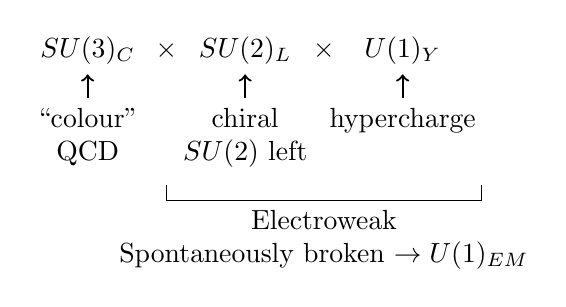
\begin{tikzpicture}
        \node at (0,0) {\(SU(3)_C\)};
        \node at (1,0) {\(\times\)};
        \node at (2,0) {\(SU(2)_L\)};
        \node at (3,0) {\(\times\)};
        \node at (4,0) {\(U(1)_Y\)};
        \draw[<-, thick] (0,-0.3) -- (0,-0.6) node[below, align=center] {``colour''\\QCD};
        \draw[<-, thick] (2,-0.3) -- (2,-0.6) node[below, align=center] {chiral \\\(SU(2)\) left};
        \draw[<-, thick] (4,-0.3) -- (4,-0.6) node[below, align=center] {hypercharge};
        \draw(1,-1.7) -- (1,-1.9) -- (5,-1.9) -- (5,-1.7);
        \node[below,align=center] at (3,-1.9) {Electroweak\\Spontaneously broken \(\rightarrow U(1)_{EM}\)};
    \end{tikzpicture}
\end{figure}

In this course we will take the conventions:
\begin{equation}
    \eta=\eta_s=\eta'=\eta_z=\eta_\theta=\eta_\gamma=\eta_e=+1
\end{equation}
The meanings of these symbols will hopefully become clear.

The course will follow the following general outline:
\begin{itemize}
    \item Symmetries (chiral, gauge, discrete)
    \item Spontaneous symmetry breaking
    \item Electroweak interactions
    \item QCD
    \item Effective field theories
\end{itemize}

\section{Chiral and Gauge symmetries}
To begin, we will review some concepts and set some notation and conventions.

\subsection{Chiral symmetry}
Consider a spin \(\frac{1}{2}\) Dirac fermion with spinor field \(\psi\) that satisfies the Dirac equation:
\begin{equation}
    (i\slashed{\partial}-m)\psi \qq{where} \slashed{\partial} = \gamma^\mu\partial_\mu
\end{equation}
The adjoint \(\overline{\psi}\) satisfies:
\begin{equation}
    \overline{\psi}(i\overleftarrow{\slashed{\partial}}+m)=0 \quad \text{where } \overleftarrow{\partial} \text{ acts to the left.}
\end{equation}
The Dirac matrices \(\gamma^\mu\) satisfy \(\{\gamma^\mu,\gamma^\nu\}=2g^{\mu\nu}\identity\), where \(g_{\mu\nu}=\operatorname{diag}(1,-1,-1,-1)\) is the Minkowski metric. We also define \(\gamma^5=-i\gamma^0\gamma^1\gamma^2\gamma^3\), from which we can deduce \(\left( \gamma^5 \right)^2=1\) and \(\{\gamma^5,\gamma^\mu\}=0\).

The chiral (or Weyl) representation is given by:
\begin{equation}
    \gamma^0 = 
    \begin{pmatrix}
        0 & \identity \\
        \identity & 0
    \end{pmatrix}, \quad
    \gamma^i =
    \begin{pmatrix}
        0 & \sigma^i \\
        -\sigma^i & 0
    \end{pmatrix}, \quad
    \gamma^5 = 
    \begin{pmatrix}
        \identity & 0 \\
        0 & -\identity
    \end{pmatrix}
\end{equation}
where the \(\sigma^i\) are the Pauli matrices.

It is useful to consider the massless Dirac equation \(\slashed{\partial}\psi=0\). We have \(\slashed{\partial}\gamma^5\psi=0\). We can define the projection operators \(P_{L,R} =\frac{1}{2}(1\pm\gamma^5)\), and define \(\psi_{L,R} = P_{L,R}\psi\), from which we can deduce \(\overline{\psi}_{L,R}=\overline{\psi}P_{R,L}\). It is easy to verify that these are projection operators:
\begin{equation}
    P_{L,R}^2=P_{L,R}, \quad P_LP_R=P_RP_L=0, \quad P_L+P_R=1
\end{equation}
In the chiral representation:
\begin{equation}
    P_L = 
    \begin{pmatrix}
        0 & 0 \\
        0 & \identity
    \end{pmatrix}, \quad
    P_R = 
    \begin{pmatrix}
        \identity & 0 \\
        0 & 0
    \end{pmatrix}
\end{equation}
So we can see that in the chiral representation, \(\psi_{L,R}\) only contain respective the lower or upper two components of the spinor degrees of freedom. Also, \(\gamma^5\psi_{L,R}=\pm\psi_{L,R}\), so \(\psi_{L,R}\) have definite chirality, by which we mean they are eigenvectors of \(\gamma^5\).

The massless Dirac equation has \(U(1)_L\times U(1)_R\) chiral symmetry:
\begin{equation}
    \psi_L\rightarrow e^{i\alpha_L}\psi_L,\quad \psi_R\rightarrow e^{i\alpha_R}\psi_R
\end{equation}
\begin{equation}
    \overline{\psi}_{L,R} \rightarrow \overline{\psi}_{L,R} e^{-i\alpha_{L,R}}
\end{equation}

Consider the Dirac Lagrangian where we now include mass:
\begin{align}
    \mathcal{L} &= \overline{\psi}(i\slashed{\partial}-m)\psi\\
    &= \overline{\psi}_Li\slashed{\partial}\psi_L
    + \overline{\psi}_Ri\slashed{\partial}\psi_R
    - m (\overline{\psi}_R\psi_L + \overline{\psi}_L\psi_R )
\end{align}
We see that the kinetic term is invariant under a chiral left and right transformation, but the mass term breaks this symmetry explicitly. It converts it into a vector symmetry. We require \(\alpha_L=\alpha_R\), so:
\begin{equation}
    U(1)_L\times U(1)_R \rightarrow U(1)_V
\end{equation}

\subsubsection{Aside on the Dirac field}
\lecture{18/01/16}
Consider the usual plane-wave decomposition of the Dirac field:
\begin{equation}
    \psi(x) = \sum_{p,s}\left[ b^s(p)u^s(p)e^{-ip\vdot x} + \herm{d^s}(p)v^s(p)e^{ip\vdot x}\right]
\end{equation}
where \(\sum_p = \lint{p}\), \(u^s\) and \(v^s\) are 4-component spinors such that \((\slashed{p}-m)u = 0\), \((\slashed{p}+m)v = 0\), \(\herm{b}\) and \(\herm{d}\) are operators that create positive and negative frequency particles respectively, and \(s = \pm\frac{1}{2}\). In the chiral representation:
\begin{equation}
    u^s(p) = 
    \begin{pmatrix}
        \sqrt{p\vdot\sigma} \xi^s \\ \sqrt{p\vdot\bar{\sigma}} \xi^s
    \end{pmatrix}
    ,\quad
    v^s(p) = 
    \begin{pmatrix}
        \sqrt{p\vdot\sigma} \zeta^s \\ -\sqrt{p\vdot\bar{\sigma}} \zeta^s
    \end{pmatrix}
\end{equation}
where \(\xi\) and \(\zeta\) are two component spinors, \(\xi^{\frac{1}{2}} = {1 \choose 0}\), \(\xi^{-\frac{1}{2}} = {0 \choose 1}\) and we will discuss \(\zeta^s\) later, \(\sigma = (1,\sigma^i\), \(\bar{\sigma} = (1,-\sigma_i)\). Note that \(\sqrt{p\vdot\sigma}\) should be dealt with in its eigenvector basis. For example if we rotate spatial co-ordinates so that \(\vb{p}\) is pointed along \(\vb{e}_3\), then we have:
\begin{equation}
    \sqrt{p\vdot\sigma} = \sqrt{p^0-p^3}\frac{1+\sigma^3}{2} + \sqrt{p^0+p^3}\frac{1-\sigma^3}{2}
\end{equation}

Helicity \(h\) is defined as the projection of the angular momentum onto the linear momentum direction:
\begin{equation}
    h = \vb{J}\vdot\vu{p} = \vb{S}\vdot\vu{p} \qq{where}
    \begin{matrix}
        \vb{J} = -i\vb{r}\times\grad+\vb{S} \\
        S_i = -\frac{i}{4}\epsilon_{ijk}\gamma^j\gamma^k = - \frac{1}{2}
        \begin{pmatrix}
            \sigma^i & 0 \\
            0 & \sigma^i
        \end{pmatrix}
    \end{matrix}
\end{equation}
Note that \(\gamma^5S^i = \frac{1}{2}\gamma^0\gamma^i = S^i\gamma^5\), so for the massless Dirac field we have:
\begin{align}
    &\slashed{p} u = 0 \\
    \implies& \frac{\gamma^5\gamma^0}{p}(\gamma^0p^0-\vb*{\gamma}\vdot\vb{p})u^s(p) = 0 \\
    \implies& (\gamma^5 - 2\vb{S}\vdot\vu{p})u^s(p) = 0 \\
    \implies& hu^s(p) = \frac{1}{2}\gamma^5u^s(p)
\end{align}
If we define \(u^s_{\text{L,R}} = \frac{1}{2}(1\mp\gamma^5)u^s\) then we have \(hu^s_{\text{L,R}} = \mp\frac{1}{2}u^s_{\text{L,R}}\), i.e. eigenvectors with \(
\begin{matrix}
    \text{positive} \\ \text{negative}
\end{matrix}
\) helicity are \(
\begin{matrix}
    \text{right} \\ \text{left}
\end{matrix}
\) handed.

Helicity is \emph{not} a Lorentz invariant for massive particles, but for massless particles, helicity and chirality coincide.

\subsection{Gauge symmetry}
We consider a \(U(1)_v\) transformation and promote \(\alpha\) to a function of spacetime position \(\alpha(x)\) (we say that we \emph{gauge} the \(U(1)_v\) symmetry). The kinetic term is no longer invariant under an arbitrary transformation:
\begin{equation}
    \overline{\psi}i\slashed{\partial}\psi \rightarrow \overline{\psi}i\slashed{\partial}\psi \overline{\psi}\gamma^\mu\psi\partial_\mu\alpha(x)
\end{equation}
To counter this, we introduce a covariant derivative \(D_\mu\) such that \(D_\mu\psi\rightarrow e^{i\alpha(x)}D_\mu\psi\), and a \emph{gauge field} \(A_\mu(x)\) such that \(A_\mu \rightarrow A_\mu - \frac{1}{g}\partial_\mu\alpha\), and set:
\begin{equation}
    D_\mu\psi = (\partial_\mu + igA_\mu)\psi
\end{equation}
We then see that \(\overline{\psi}i\slashed{D}\psi \rightarrow \overline{\psi}i\slashed{D}\psi\). If we replace partial derivatives with covariant derivatives we obtain in the Lagrangian a kinetic term for the gauge fields \(\mathcal{L}_{\text{gauge}} = - \frac{1}{4}F_{\mu\nu}F^{\mu\nu}\) where \(F_{\mu\nu} = \partial_\mu A_\nu - \partial_\nu A_\mu\).

\subsubsection{Non-abelian gauge symmetry}

We generalise the transformations to:

\begin{equation}
    \psi_i(x) \rightarrow U_{ij}(x)\psi_j(x) = \exp(it^a\theta_a(x))_{ij}\psi_j(x)
\end{equation}
\begin{equation}
    \overline{\psi}_i(x) \rightarrow \overline{\psi}_j(x) \herm{U}_{ij}(x) = \overline{\psi}_j(x)\exp(-it^a\theta_a(x))_{ji}
\end{equation}
where \(\psi_i\) is a field transforming in an \(n\)-dimensional representation \(R\) of a unitary group, \(t^a\) are the Hermitian generators in that representation, and \(i,j\in\{1,\dots,n\}\).

\lecture{20/01/16}
The \(t^a\) form a Lie algebra. We define the structure constants \(f^{abc}\) by \([t^a,t^b] = i f^{abc}t^c\), and the Dynkin index \(T(R)\) of \(R\) by \(\Tr(t^at^b)=T(R)\delta^{ab}\).

In the standard model, the fermions belong to trivial (\(n=1\)) or fundamental representations.

In analogy to the abelian case, we define a covariant derivative as follows:
\begin{equation}
    (D_\mu)_{ij} = \partial_\mu\delta_{ij} + ig(t^aA^a_\mu)_{ij}
\end{equation}
Under a gauge transformation, we have \((D_\mu\psi)_i\rightarrow (U(x)D_\mu\psi)_i\). We also define the field-strength tensor \(F^a_{\mu\nu}\) by:
\begin{equation}
    [D_\mu,D_\nu] = igt^aF^a_{\mu\nu}
\end{equation}
where we have dropped the \(i,j\) indices. We can write this as:
\begin{equation}
    F^a_{\mu\nu} = \partial_\mu A^a_\nu - \partial_\nu A^a_\mu - gf^{abc}A^b_\mu A^c_\nu
\end{equation}
The contribution of the field-strength tensor to the lagrangian is:
\begin{equation}
    \mathcal{L}_g = -\frac{1}{4}F^a_{\mu\nu}F^{a\,\mu\nu} = -\frac{1}{2}\Tr F_{\mu\nu}F^{\mu\nu}
\end{equation}

\subsection{Types of symmetry}
Symmetries can manifest themselves in a number of different ways:
\begin{itemize}
    \item Symmetries can exist in both classical physics and quantum physics. Such symmetries are said to be \emph{intact}. Examples in the Standard Model include \(U(1)_{\text{EM}}\) and \(SU(3)_{\text{C}}\).
    \item A symmetry can exist in classical physics, but be broken by quantum effects. It is said to be broken by an \emph{anomaly}. In the Standard Model, the global axial symmetry \(U(1)_{\text{A}}\) is anomalous.
    \item If a symmetry holds for some terms in the Lagrangian but not others, it is said to be \emph{broken explicitly}. It may still be an appropriate symmetry to consider if the symmetry breaking terms are small. In the standard model, the global isospin symmetry relating up and down quarks (a global \(SU(2)\)) is only approximate, as it is broken by differences in mass and charge.
    \item If a symmetry is respected by the Lagrangian but not by the vacuum, then it is said to be \emph{spontaneously broken} or to be a \emph{hidden symmetry}. These symmetries have important physical consequences. In the standard model, \(SU(2)_{\text{L}} \times U(1)_{\text{Y}}\) is spontaneously broken to \(U(1)_{\text{EM}}\) by the Higgs mechanism.
\end{itemize}

\section{Discrete symmetries}
There are three important discrete symmetries that we must consider:
\begin{description}
    \item[Parity] (\(P\)): \((t,\vb{x})\rightarrow(t,-\vb{x})\)
    \item[Time reversal] (\(T\)): \((t,\vb{x})\rightarrow(-t,\vb{x})\)
    \item[Charge conjugation] (\(C\)): particles \(\rightleftharpoons\) antiparticles
\end{description}
Parity and time reversal are spacetime symmetries.

Gauge theories with vector-like couplings to fermions (e.g. QED, QCD) are invariant under \(P\) and \(C\). However, theories that couple only to left-handed fermions (e.g. weak interactions) are not. In fact the combination \(CP\) is violated in the weak interaction. The \(CPT\) theorem states that the combination \(CPT\) must be conserved, so we have that the weak interaction violates \(T\) as well. 

To fully understand these statements, we first investigate the consequences of theories that do respect \(C\), \(P\) and \(T\).

\subsection{Spacetime symmetry operators}
A general Poincar\'e transformation is a change of coordinate frame:
\begin{equation}
    x^\mu \rightarrow x'^\mu = \Lambda^\mu_\nu x^\nu + a^\mu
\end{equation}
Proper Lorentz transformations have \(\det\Lambda = +1\). Parity and time reversal are improper Lorentz transformations:
\begin{align}
    \text{Parity has } \Lambda_\nu^\mu &= \mathbb{P}^\mu_\nu = 
    \begin{pmatrix}
        1 \\
        &-1\\
        &&-1\\
        &&&-1
    \end{pmatrix} \\
    \text{Time reversal has } \Lambda_\nu^\mu &= \mathbb{T}^\mu_\nu = 
    \begin{pmatrix}
        -1 \\
        &1 \\
        &&1\\
        &&&1
    \end{pmatrix}
\end{align}

\begin{theorem}[Wigner]
    If physics is invariant under \(\psi\rightarrow\psi'\) where \(\psi,\psi'\) are vectors in some Hilbert space \(\mathcal{H}\), then there is an operator \(W\) such that \(\psi'=W\psi\) such that:
    \begin{itemize}
        \item either \(W\) is unitary and linear:
            \begin{equation}
                (W\phi,W\psi) = (\phi,\psi)
                \quad
                W(\alpha\phi + \beta\psi) = \alpha W\phi + \beta W\psi
            \end{equation}
        \item or \(W\) is anti-unitary and anti-linear:
            \begin{equation}
                (W\phi,W\psi) = (\phi,\psi)^*
                \quad
                W(\alpha\phi + \beta\psi) = \alpha^* W\phi + \beta^* W\psi
            \end{equation}
    \end{itemize}
    where \(\alpha,\beta\in\CC\) and \(\phi,\psi\in\mathcal{H}\).
\end{theorem}

Consider an infinitesimal (proper) Poincar\'e transformation \(\Lambda^\mu_\nu = \delta^\mu_\nu + w^\mu_\nu\), \(a^\mu = \varepsilon^\mu\), where \(w^\mu_\nu\) and \(\varepsilon^\mu\) are small parameters.

\lecture{22/01/16}
We can expand the operator \(W\) corresponding to this transformation as:
\begin{equation}
    W(\Lambda,a) = W(1+\omega,\varepsilon) = 1 + \frac{i}{2}\omega_{\mu\nu}J^{\mu\nu}-i\varepsilon_\mu p^\mu
    \tag{\(*\)}
    \label{infipoincare}
\end{equation}
where \(p^0\) is the Hamiltonian, \(p^i\) is the linear momentum operator (generating translations), \(\vb{J}=(J^{23},J^{31},J^{12})\) is the angular momentum operator (generating rotations), and \(\vb{k}=(J^{01},J^{02},J^{03})\) (generating boosts).

We have \(\hat{P} = W(\mathbb{P},0)\) and \(\hat{T} = W(\mathbb{T},0)\). It is easy to verify that:
\begin{equation}
    \hat{P}W\hat{P}^{-1} = W(\mathbb{P}\omega\mathbb{P}^{-1},\mathbb{P}\varepsilon)
    ,\quad
    \hat{T}W\hat{T}^{-1} = W(\mathbb{T}\omega\mathbb{T}^{-1},\mathbb{T}\varepsilon)
\end{equation}
If we insert \eqref{infipoincare} into these equations, and equate coefficients of \(\varepsilon_\mu\) on both sides, we obtain:
\begin{equation}
    \hat{P}ip^\mu\hat{P}^{-1} = i\mathbb{P}\indices{_\nu^\mu}p^\nu
    ,\quad
    \hat{T}ip^\mu\hat{T}^{-1} = i\mathbb{T}\indices{_\nu^\mu}p^\nu
\end{equation}
In particular, if we look at \(\mu=0\), we have:
\begin{equation}
    \hat{P}iH\hat{P}^{-1} = iH
    ,\quad
    \hat{T}iH\hat{T}^{-1} = -iH
\end{equation}
Now let \(\psi\) be an energy eigenstate with energy \(E\), \(\braket{\psi}{iH\psi}=iE\), and suppose that \(P\) and \(T\) are symmetries of our theory. Then we should have \(\hat{P}\psi\) and \(\hat{T}\psi\) are also eigenstates with the same energy \(E\). It turns out this is consistent with \(\hat{P}\) being linear and unitary:
\begin{equation}
    \braket{\hat{P}\psi}{iH\hat{P}\psi} = \braket{\hat{P}\psi}{\hat{P}iH\psi} = \braket{\psi}{iH\psi} = iE
\end{equation}
and \(\hat{T}\) being antilinear and antiunitary:
\begin{equation}
    \braket{\hat{T}\psi}{iH\hat{T}\psi} = -\braket{\hat{T}\psi}{\hat{T}iH\psi} = -\braket{\psi}{iH\psi}^* = -(iE)^* = iE
\end{equation}

\subsection{Parity}
\subsubsection{Scalar fields}
Recall that a quantum scalar field \(\phi(x)\) can be written as:
\begin{equation}
    \phi(x) = \sum_p\left[ a(p)e^{-ip\vdot x} + \herm{c}(p)e^{ip\vdot x} \right]
\end{equation}
where \(a(p)\) annihilates a particle with momentum \(p\), and \(\herm{c}(p)\) creates an antiparticle with momentum \(p\). In general parity maps momentum states in the following way:
\begin{equation}
    \ket{p}\rightarrow{\eta^a}^*\ket{p_P}
\end{equation}
where \(p = (p^0,\vb{p})\), \(p_P = (p^0,-\vb{p})\), and \({\eta^a}^*\) is some complex phase. If we assume that the vacuum is conserved under parity transformations \(\hat{P}\ket{0} = \ket{0}\), then, since \(\ket{p}=\herm{a}(p)\ket{0}\), we have:
\begin{equation}
    \hat{P}\herm{a}(p)\hat{P}^{-1} = \herm{a}(p_P){\eta^a}^*
\end{equation}
To conserve normalisations, we have:
\begin{equation}
    \hat{P}a(p)\hat{P}^{-1} = \eta^a a(p_P)
\end{equation}
Similarly:
\begin{equation}
    \hat{P}\herm{c}(p)\hat{P}^{-1} = {\eta^c}^* \herm{c}(p_P)
    \qq{and}
    \hat{P}c(p)\hat{P}^{-1} = \eta^c c(p_P)
\end{equation}
Using these expressions, we can deduce how \(\phi(x)\) transforms under a parity transformation:
\begin{align}
    \hat{P}\phi(x)\hat{P}^{-1} 
    &= \sum_p \left[ \hat{P}a(p)\hat{P}^{-1}e^{-ip\vdot x} + \hat{P}\herm{c}(p)\hat{P}^{-1}e^{+ip\vdot x} \right] \\
    &= \sum_p \left[ \eta^aa(p_P)e^{-ip\vdot x} + {\eta^c}^*\herm{c}(p_P)e^{+ip\vdot x} \right] \\
    &= \sum_{p_P} \left[ \eta^aa(p)e^{-ip_P\vdot x} + {\eta^c}^*\herm{c}(p)e^{+ip_P\vdot x} \right] \\
    &= \sum_p \left[ \eta^aa(p)e^{-ip\vdot x_P} + {\eta^c}^*\herm{c}(p)e^{+ip\vdot x_P} \right] \\
\end{align}
If \(\eta^a \ne {\eta^c}^*\), then it is possible to deduce that \([\phi(x),\phi^P(y)]\) does not vanish for for spacelike \(x-y\), which we must require. Thus we set \(\eta_P = \eta^a = {\eta^c}^*\), and we have:
\begin{equation}
    \hat{P}\phi(x)\hat{P}^{-1} = \eta_P\phi(x_P)
\end{equation}
\(\eta_P\) is often called the \emph{intrinsic parity} of \(\phi\).

For real fields, we have \(c(p) = a(p)\), so \(\eta^c = \eta^a = {\eta^c}^* \in \RR\). Further, to preserve normalisation we require \(|\eta_P| = 1\), so we have two possible cases:
\begin{itemize}
    \item \(\eta_P = 1\). Such fields are said to be \emph{scalar}.
    \item \(\eta_P = -1\). Such fields are said to be \emph{pseudoscalar}.
\end{itemize}

For complex fields, \(\eta_P\) may not be real, but if there is a conserved charge \(Q\), then we can express \(\eta_P\) in terms of \(Q\).

\subsubsection{Vector fields}
Consider a vector field \(V^\mu(x)\). We have:
\begin{equation}
    \hat{P}V^\mu\hat{P}^{-1} = -\eta_P \mathbb{P}\indices{^\mu_\nu}V^\nu(x_P)
\end{equation}
\emph{Vectors} have \(\eta_P = -1\), and \emph{axial vectors} have \(\eta_P = +1\).

\end{document}
